\documentclass{article}

\usepackage{graphicx}
\usepackage{tikz}
\usetikzlibrary{shapes.geometric, arrows} 
\usepackage{hyperref}
\hypersetup{
    colorlinks=true,
    linkcolor=blue,
    filecolor=magenta,      
    urlcolor=cyan,
    pdftitle={Overleaf Example},
    pdfpagemode=FullScreen,
}
\usepackage{titlesec}
\usepackage{geometry}
 \geometry{
 a4paper,
 total={170mm,257mm},
 left=20mm,
 top=20mm,
 }

%flowchart
\tikzstyle{startstop} = [rectangle, rounded corners, minimum width=3cm, minimum height=1cm, text centered, draw=black, fill=red!30]
\tikzstyle{io} = [trapezium, trapezium left angle=70, trapezium right angle=110, minimum width=3cm, minimum height=1cm, text centered, draw=black, fill=blue!30]
\tikzstyle{process} = [rectangle, minimum width=3cm, minimum height=1cm, text centered, draw=black, fill=orange!30]
\tikzstyle{decision} = [diamond, minimum width=3cm, minimum height=1cm, text centered, draw=black, fill=green!30]
\tikzstyle{arrow} = [thick,->,>=stealth]

\title{Unit 15 LO2}
\author{Chris}
\date{}

\begin{document}

\maketitle
\tableofcontents
\break

\section{P3 Create a design for an identified game concept}
We have been tasked in the previous Units to create a game for a food retailer. They are a fresh and modern company who are aware of moderen digital marketing techniques.
They are clear that they want to have a game developed which will be used as a part of their advertising campaigns. To that end they want to have a game developed that incorporates their branding and mascot, a food ninja.
The artifacts in the game must relate to their fast food outlets and the gameplay must be fun and engaging and reflect their healthy attitudes to food. 

The game is to be targetted at a younger audience and should have a an easy to pickup layout, meaning that the game play should be something most players will have played previously. To that end a platformer has been requested. 

\subsection{Game elements}
\subsubsection{navigation}
The navigation in the game is done by providing important information to the player to the player by either using a Heads Up Display(HUD) for example compasses,maps or arrow signs. Both of these methods are helpful in games and their use depends on game's genre and how the game designers want the player to experience the game.

The HUD said by Greg Wilson in the article \textit{Off With Their HUDs} described HUD as "A collection of persistent onscreen elements whose purpose is to indicate player status. HUD elements can be use to show, among many other things, how much health the player has, in which direction the player is heading, or where the player ranks in a race" 



\subsubsection{scoring}
Scoring in games are key component of game mechanics and it provides a mechanic where the players get rewarded with point value whenever they accomplish a task in the game.   

\subsubsection{movement}
The movement for the game is
Moving a character is so common in games that players and designers often take it for granted. However, while it can be tempting to use the default movement options in a game engine, designing great movement can make simply controlling a character fun. 

\subsubsection{interaction/controls}
three main principles for good game controls are:
\begin{enumerate}
	\item Accessibility - the controls should be easy to learn and use, and take into account physical and cognitive limitations
	\item Intent Communication - the controls should communicate the player's intent in a way the player expects and create a feeling of full control
	\item Expression Space - the controls should give the player enough expression so that they players can master while also keep a sufficient level of variety.
\end{enumerate}

Accessibility 
If we want our controls to be easy to learn and use we need to take into account everyone physical and cognitive limitation 

\subsubsection{conveying information}
Classic tutorials are one of the worst ways to convey information to the players about the game. These levels are are often some of the least fun parts of the entire game and some are un-skippable these are worst, making them not every effective at their job.

\subsubsection{sound}
Designing Sounds in a game are:
Talking about various sounds found in a particular game, those could be generalised to the following types: 
\begin{enumerate}
	\item Sound Effects - The sounds the objects in the game game make
	\item Music -  A game has 2 or 3 main themes for example menu music and the level music
	\item Voice-overs - are the character lines
\end{enumerate}

\subsubsection{levels}
Their will be 5 levels in our game and all of them are going to themed after our clients food. Each level is unique and different from each other 

\subsubsection{enemies}
The eniemes of the game will be small and easy to hit since this game is designed for kids and young teens. The height of these mobs will be half height of the player character. We do this because it makes it easier for our target audience to understand our game and theconcepts to the gamer. 


\subsubsection{problem solving}
The is small amount of problem solving in our game because we are 2D platformer and we have small traps and enemies for the player to get around. The traps are disguised to hide/blend them into scenario so that they "get" the player, the traps do look different enough that the players can detect and dodge the traps.

\subsection{Interface design}
\subsubsection{layout}
The Layout out of each levels is going to be designed to promoted a 

\subsubsection{colour palette}
The colour palette is going to be bright eye catching colours for the  

\subsubsection{text styles}
The text style for the game is going to cartoony style to entise our target audience to click and download our clients game. 

\subsubsection{sound}
The sound for the game is basic as can be and will be kept to minium since they are uneccessery and execpt the game to be muted when playing since it will be on a phone

\subsubsection{stage/scene}
Stage in the game is going ot simplre and 

\subsubsection{actions}
Actions that will be done are fighting enimes and 


\section{P4 Produce a logic structure for the identified game concept}
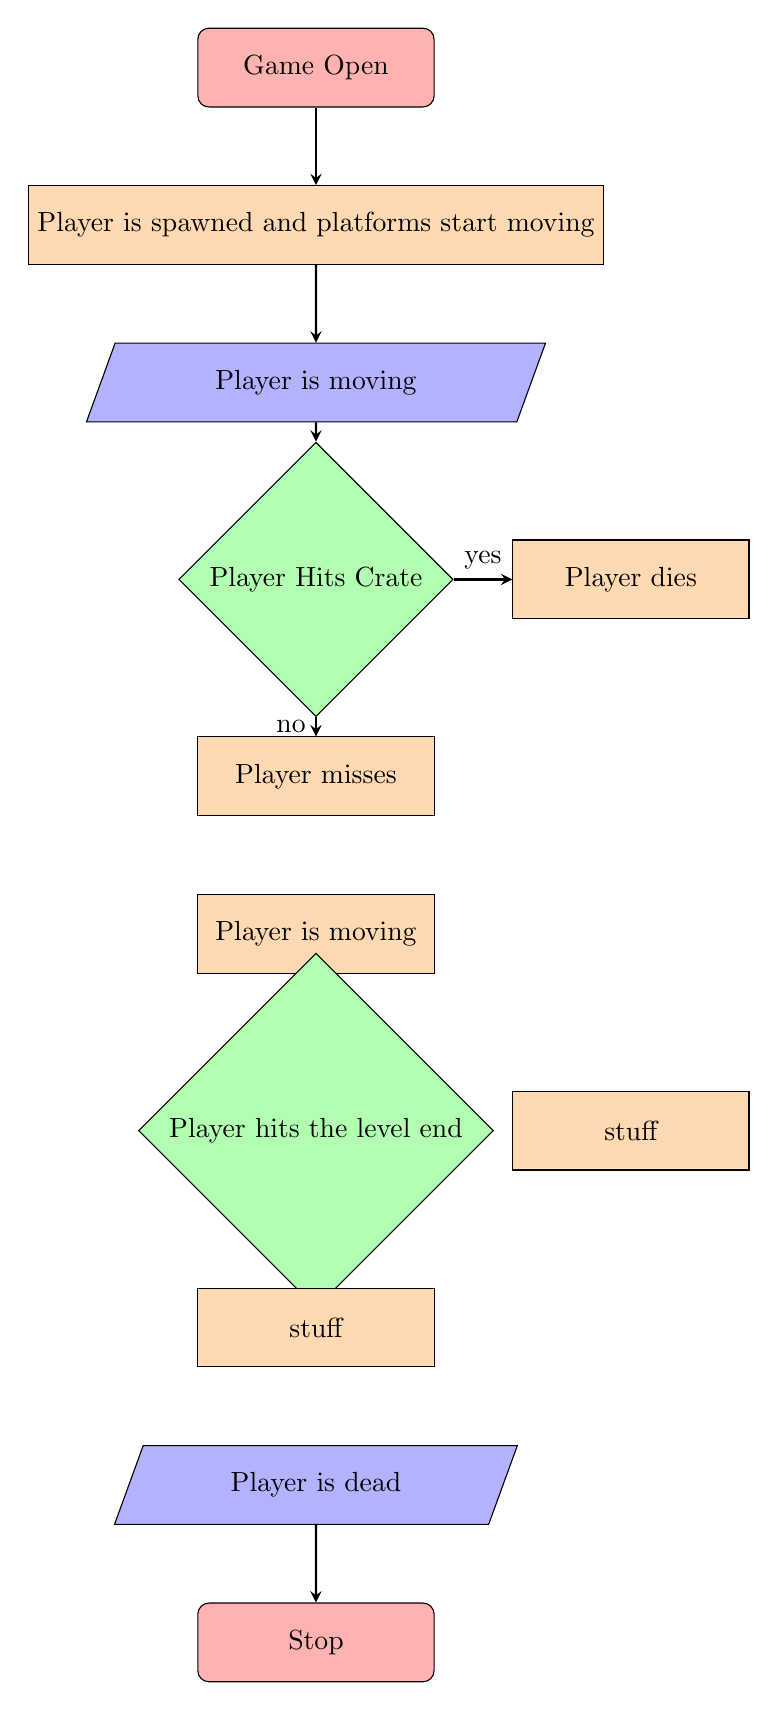
\begin{tikzpicture}[node distance=2cm]
	\node (start) [startstop] {Game Open};
	\node (proc1) [process, below of=start] {Player is spawned and platforms start moving};
		\draw [arrow] (start) -- (proc1);
	\node (in1) [io, below of=proc1] {Player is moving};
		\draw [arrow] (proc1) -- (in1);
	\node (dec1) [decision, below of=in1, yshift=-0.5cm] {Player Hits Crate};
		\draw [arrow] (in1) -- (dec1);
	\node (proc2a) [process, below of=dec1, yshift=-0.5cm] {Player misses};
		\draw [arrow] (dec1) -- node[anchor=east] {no} (proc2a);
	\node (proc2b) [process, right of=dec1, xshift=2cm] {Player dies};
		\draw [arrow] (dec1) -- node[anchor=south] {yes} (proc2b);
	\node (proc3) [process, below of=proc2a] {Player is moving};
	\node (dec2) [decision, below of=proc3,yshift=-0.5cm] {Player hits the level end};
	\node (proc3a) [process, right of=dec2, xshift=2cm] {stuff};
	\node (proc3b) [process, below of=dec2, yshift=-0.5cm] {stuff};

	\node (out1) [io, below of=proc3b] {Player is dead};
	\node (stop) [startstop, below of=out1] {Stop};
		\draw [arrow] (out1) -- (stop);
	
\end{tikzpicture}

include diagrams to give evidence about the structure for the game. Give clear definition of objectives of the game. Flow chart showing the flow of the game through single or multiple layers with single or multiple players.

Include visualisation or written planetary designs or a combination of both and including alternatives, together with diagrams such as flowcharts.






\section{M2 Prepare alternative interface designs for the identified game concept}
Alternative interface designs is a hudless design. This done by having these elements intergrated into the world for the health,score and timers. The hud can be easily show in the game world by having visual signs to the uaser, this can be done by having a bars or having the player charater getting more visually hurt. The score system can be shown either by charater looks "increasing"
Prepare alternative interface designs to the one identified in P3. The alternative designs must contain enough detail to enable them to be understood by a third party. Evidence can be extension of P3 and be presented as additional visualisations or written explanatory designs, or a combination of both.




\section{D1 Justify the design rational for the identified game concept}


Justify the designs choices and explain why they are suitable for the identified audience and purpose of the game concept. Evidence can be an extension of P3 and M2, and can be addition to the design documentation, a presentation or a report, but should reference the designs submitted.



\end{document}
